\documentclass[titlepage,a4paper,11pt,oneside]{book} % Document Class

% Font styling
\usepackage{mathptmx}
\usepackage[T1]{fontenc}
% Margins
\usepackage[margin=3cm]{geometry}

% Graphics
\usepackage{graphicx}

% Code snippets
\usepackage[dvipsnames]{xcolor}
\usepackage{listings}
\lstloadlanguages{Ruby}
\lstset{%
basicstyle=\ttfamily\color{black},
commentstyle = \ttfamily\color{red},
keywordstyle=\ttfamily\color{blue},
stringstyle=\color{orange}}

% Bibliography
\usepackage{cite}
\usepackage{natbib}
\bibliographystyle{agsm}
%\usepackage[nottoc,numbib]{tocbibind}

% Abbreviations
%\usepackage[refpage]{nomencl}
\usepackage[intoc]{nomencl}
\renewcommand{\nomname}{Abbreviations}
\makenomenclature

%Meta data
\author{Daniel James Wilson}
\title{Progress Monitoring Web Application}
\date{\parbox{\linewidth}{\centering%
  \today\endgraf\bigskip
  Supervisor:\\
  Dr Moi Hoon Yap}}


% Document
\begin{document}
\frontmatter % roman numbers
\maketitle

\chapter{Acknowledgments}
I'd like to express my gratitude to my parents, for their support throughout my three years of studying at university, my other half, Grace Day, for proof reading this dissertation, and my supervisor Dr Moi Hoon Yap for her invaluable support and advise with this dissertation.

\chapter{Abstract}
This is a report on the development of a fitness monitoring applicatoin and why fitness monitoring applications are important the the everyday human.

\tableofcontents

\pagebreak
\addcontentsline{toc}{chapter}{List of Figures}
\listoffigures
\pagebreak

\pagestyle{empty}
\printnomenclature[2cm]

\mainmatter % normal numbers
\chapter{Introduction}
\label{sec:mainIntro}
\subsection{Fitness applications}
Fitness applications are important because it gives people a way to monitor how they are getting on with their health. Keeping fit and getting healthy is an everlasting venture, and you will only notice improvements over a long period. Although, while you may not see a physical change, you are improving with every trip to the gym. What fitness monitor applications do is allow you to track what did at the gym and how well you did. For example, if you went on the treadmill, you could track how long it took you to run a mile. Next time you go on the treadmill, you will log your mile time again and see if you have improved. It also gives that edge of motivation. By showing you how well you are doing it gives you the motivation to keep at it. If you are not doing so great, it will allow you to see where you need to improve.\\

\subsection{Benefits of being fit and healthy}

\subsection{Applications}
Mobile and web applications are on the rise. People are constantly on their phones interacting with their applications, be it a native mobile application or a web based application. Applications are usefully because they usually do one or two tasks really well. Be that; recording notes or tracking your blood sugar levels. They allow the user to track information and keep it all organised. With this information, the application will be able to display back to the user in an orderly fashion; whether that is in the forma of table listing all their previous expenses, or a graph showing how much they have spent in certain categories.

\subsection{Recur}
Recur is the fitness application that is being documented in this dissertation. It focuses on three main aspects of fitness. These are:

\begin{enumerate}
\item {Current and goal weight}
\item {Fitness specific goals}
\item {Fitness log}
\end{enumerate}

\noindent
By keeping the application down to these three features, it will allow the users to keep focused and not get distracted by other, unnecessary aspects. It will be displayed in a modern, minimalistic design and built using up to date technologies (more on this in the development chapter \ref{sec:dev} on page \pageref{sec:dev}).\\

\subsection{Learnings}
A number of things will be learnt during the building of this application. The design stage will have to take into account user accessibility. This covers catering you design for the visually impaired and making the website as user friendly as possible. The development chapter cover the learnings of using a new MVC framework, building and authentication system, and securing it from attacks. In the testing chapter, it teaches how to write tests for test driven development.\\

\subsection{Chapters}
This dissertation will cover the whole process behind the building of the progress monitoring web application. The application is for monitoring the users fitness progress. It shall allow a user to track their current and goal weight, any goals they may want to achieve, and a diary of fitness entries. The application will focus on these three main points only to not distract the user away from their progress. Other features like social media sharing and calorie tracking will not be implemented. More information on these choices can be found in the design chapter \ref{sec:design} on page \pageref{sec:design} of the paper. The literature review chapter \ref{sec:litreview} on page \pageref{sec:litreview} will focus on current state of fitness progress monitor applications that are already available for use. It will discuss both the good and bad points about each application and what this application will do differently. The design chapter \ref{sec:design} on page \pageref{sec:design} will also cover the reasoning behind most of the design choices that were made during the planning of this application. For example, which font was chosen and why. The design chapter will also cover some development choices, such as the data structure design. After that, the development chapter \ref{sec:dev} on page \pageref{sec:dev} will talk through the development process. It will go into detail about which tools were used and why, the problems and challenges that were faced during development and how they were over come, and also deployment of the web application to the internet. Following the development chapter will be the testing chapter \ref{sec:test} on page \pageref{sec:test}. This will go over the testing methodologies and tools used in the building of the application and why they were used. It will also cover how bugs and errors picked up by the testing were overcome. The evaluation chapter \ref{sec:eval} on page \pageref{sec:eval} will cover what the outcome of the product was like compared with the original idea. It will also cover feedback from users about their and how that feedback will be acted upon. The conclusion chapter \ref{sec:conc} on page \pageref{sec:conc} will wrap up the paper with what knowledge has been gained from this build, what would have been done differently, and also possible future outcomes from the product.\\



\chapter{Literature Review}
\label{sec:litrev}
\section{Introduction}
It is known that being overweight can be a risk to your health \citep{theordre:1985}. This, along with other factors, is driving a percentage of the overweight population to try and lose weight. Most people give up on weight loss due to lack of motivation, this is what the new application all aim to fix. By allowing users to track progress through an easy to use web application, that is accessible anywhere via the internet, it will help the user maintain their motivation to keep losing the weight, and also keep the weight off once they have reached their goal weight.\\

There are already a number of weight tracking, fitness, and calorie counting applications out there on the market. Some of them offer all three services, and often a lot of other additional features, while other are more stripped down and only offer one or two. This application will focus on two or three areas to keep the user on track and not confuse them with features they do not need to worry about. The areas that my application will be focusing on are weight, goals and a fitness log.

\section{Related work}
This section will analyse a number of related websites offering a similar service to the new application. It will give a brief explanation about the service and a breakdown of the good points and the bad.

\subsection{Fitocracy}
The first application is Fitocracy \citep{fitocracy:2007}, a web and mobile application to monitor fitness. It is heavily featured, which is a plus for some people, but others can find it distracting. One of its main features is its social network site. It has a social network backend that will let the user follow your friends and give them kudos for completing certain exercises. This feature is excellent as it gives what is called a feedback loop. This is commonly used in mobile application today by having the ability to login with a social network and share progress to that social network. A social network backend is a great motivational tool but due the aim of keeping my application as simple as possible, I will not be implementing this. Fitocracy is very motivation based with features like challenges, quests, duels, and leaderboards all creating feedback loops which provide the user with constant rewards and recognition of your achievements. Again, my application will be staying very minimal so the new application won't be implementing such massive features. Instead, the new application will just have goals, which will create a small feedback loop, giving the user motivation and recognition of their goals. The main downside to Fitocracy would be the overwhelming number of features. It has so many features and options all packed into the one screen it is very overwhelming and not a nice experience to use. This is the basis of my application. To be stripped down of the unnecessary paraphernalia that surrounds applications like Fitocracy, and focus on a few key points.


\subsection{Fitbit}
Fitbit is one of the biggest fitness apps out to date. What makes it so special is that you can purchase a wristband that monitors your activity and sleep, and then wirelessly syncs your statistics with your Fitbit account. This is one of many items, known as wearable technology, which enables users to track their activity. Others include the JawboneUp \citep{jawbone:2011} and the Nike+ Fuel Band \citep{nikefuelband:2012}. This allows for less manual data entry. It counts how many steps you have taken, how many calories burnt, and how many hours sleep. Its downside is that you can only specify certain exercises. For example, working out in the gym, you cannot tell it how much you are lifting, so it cannot give you an accurate reading of how many calories you have burnt.\\

Fitbit focuses on balancing your caloric intake and expenditure to help you hit your goal weight. After inputing your details and your goal weight, it will give you a calorie intake goal. It then balances your caloric intake, by tracking your diet, and your caloric expenditure, by tracking your activity. It will then match the two and show you your calories in versus calories out. Focusing on calories in versus calories out is another popular way to lose weight. By decreasing your caloric intake and increase your caloric expenditure, you will lose weight.\\

Fitbit is very a well designed web application. It takes the popular minimalist and flat design approach. It has a really clean dashboard that consists of six cards with information right there on them. If you click on one of the cards, you will see a modal pop up with more information on that card. In the bottom right hand corner of the pop up is an arrow, clicking the arrow will take you to even more information about that specific element of the application and this page will also allow you to enter data. This is a really efficient way of laying out an application as it give the user all the information on the first page, and more information and the ability to change that information is only two clicks away.

\subsection{Nike+ FuelBand}
The Nike+ FuelBand app is a little bit different from all of the others. It uses its own measurement (Nike+ fuel) to monitor your activity. You set yourself a goal and then as you move throughout the day, your fuel will go up. It connects to your mobile device via Bluetooth so you can see your stats on the mobile application, and that syncs the data with their servers so you can see even more data on the web application. Their main goal is similar to that of the new fitness application, to keep the user motivated to get out and get exercising. They use the NikeFuel as a measurement as it is a universal way to measure all kinds of activity \citep{fuelbandpress:2013}. You can also add your friends and see how they are doing with their goals. This adds yet more motivation by being able to compete with your friends. The ability to connect with your friends is a great motivational tool but it takes away from the simplicity that the application is aiming for.

\section{Conclusion}
To conclude, my website will follow a similar simple easy to use, design to Fitbit, but with a more focused aim on motivating the user to get back into the gym. Out of the two main types of weight loss, it will focus on the fitness side. The decision was made to not implement both sides because to split the focus over two aspents would break the motivation from one focus to another. Also, the implementation of having calorie tracking would either be a big thing with a database of food types and their caloric value, or having to have the user enter both the food type and then the caloric value of that food type. This can lead to an incorrect caloric reading.\\

After seeing some of the over-complicated fitness applications with very poor user experience, the applications design was to be kept as simple as possible. Cutting down on user options and features while maintaining core, desirable features is how this will be achieved. Being a content driven application, the information needs to be readily available on the first page that the user sees, so that if they just wanted a quick view on how they are doing it would all be there as soon as they open the page.


\chapter{Design}
\label{sec:design}
\subsection{Grid design}
\citet{bertoni:2002} states that the concept of minimalist architecture is to strip everything down to its essential quality and achieve simplicity. The design of the application was to follow this simple rule. The bare essentials were the only aspects that needed to be displayed the user. The set up of the website is to have three blocks displayed in the centre of the screen, laid out on a six column grid. Grid design is important in web design as it add continuity to each page. Each page will have the relevant information in a similar position to the last, allowing the user to be able to extract the information more quickly. A grid layout also makes it easier to design for other devices. \citet{walkers:2013} found that their mobile traffic was up to 29\% in Q2 2013. From this, we can see that more and more people are browsing the internet from the mobile devices. 43\% of this traffic was from iPhones. As web designers, we need to make sure that our web applications looks as good on a 320 pixel width devices as it does on a laptop monitor. This lead to the design of the application being based on a six column grid. This was for two main reasons: the first reason to keep consistency through the sizing of different areas of the website and the second being it makes it much easier to scale the design down for mobile traffic. Due to the fact that mobile traffic is increasing, and also that the application will mainly be used on mobiles, responsiveness was very important when designing the application. It need to have the same feel on a 1920px screen as it would on a 320px mobile device screen.\\

\subsection{Wireframe and mock up}
Simple designs were sketched up in a notebook to get a feel for how each of the pages would look on both a normal monitor and a mobile devices. After sketches were complete, they were then drawn up in Sketch \citep{sketch:2013} where colour, text, and images can be added to get an even better feel for how the application is going to look and work. Once colour could be applied to the design, user accessability could be thought about. Around 8\% of men in the United Kingdom are affected by some form of colour blindness and 0.5\% of women \citep{colourBlind}. If the design was not to cater for their needs then that would be a percentage of the population that cannot use the application. Colour should never be the primary cue for information. During the design process, changes were made so that any occurrence where colour was the primary cue would also have a visual cue. For example: when the user checks off a goal, the text will have a strike through it as well as turning red. Also, a large percentage of the population have a visual impairment. A few steps were taken to keep the site safe for the visually impaired. The font size and weight is kept at a easy to read level so that it is not taking up to much space but still easily readable. Also, the colour of the font has to contrast with that of its background. From a previous design, the background of the cards and headers was very light and the font colour was too light which would be quite difficult to read for a visually impaired person. Since then, the background colour has completely changed to a darker blue and the colour of the text has been made a lighter shade of grey. As for the typeface, I went with Helvetica, as san-serif fonts are easier to read for the visually impaired. Where there is any large amount of text that the user will need to read, a line height of 1.5 will be used to make it easier to read for visually impaired people. Also, using ARIA HTML5 landmarks, such as header, footer and nav tags, will increase the usability of my website on screen readers. It is important when writing any web application to use semantic HTML that can be used easily without loading the stylesheet file.\\

\begin{figure}[!ht]
\centering
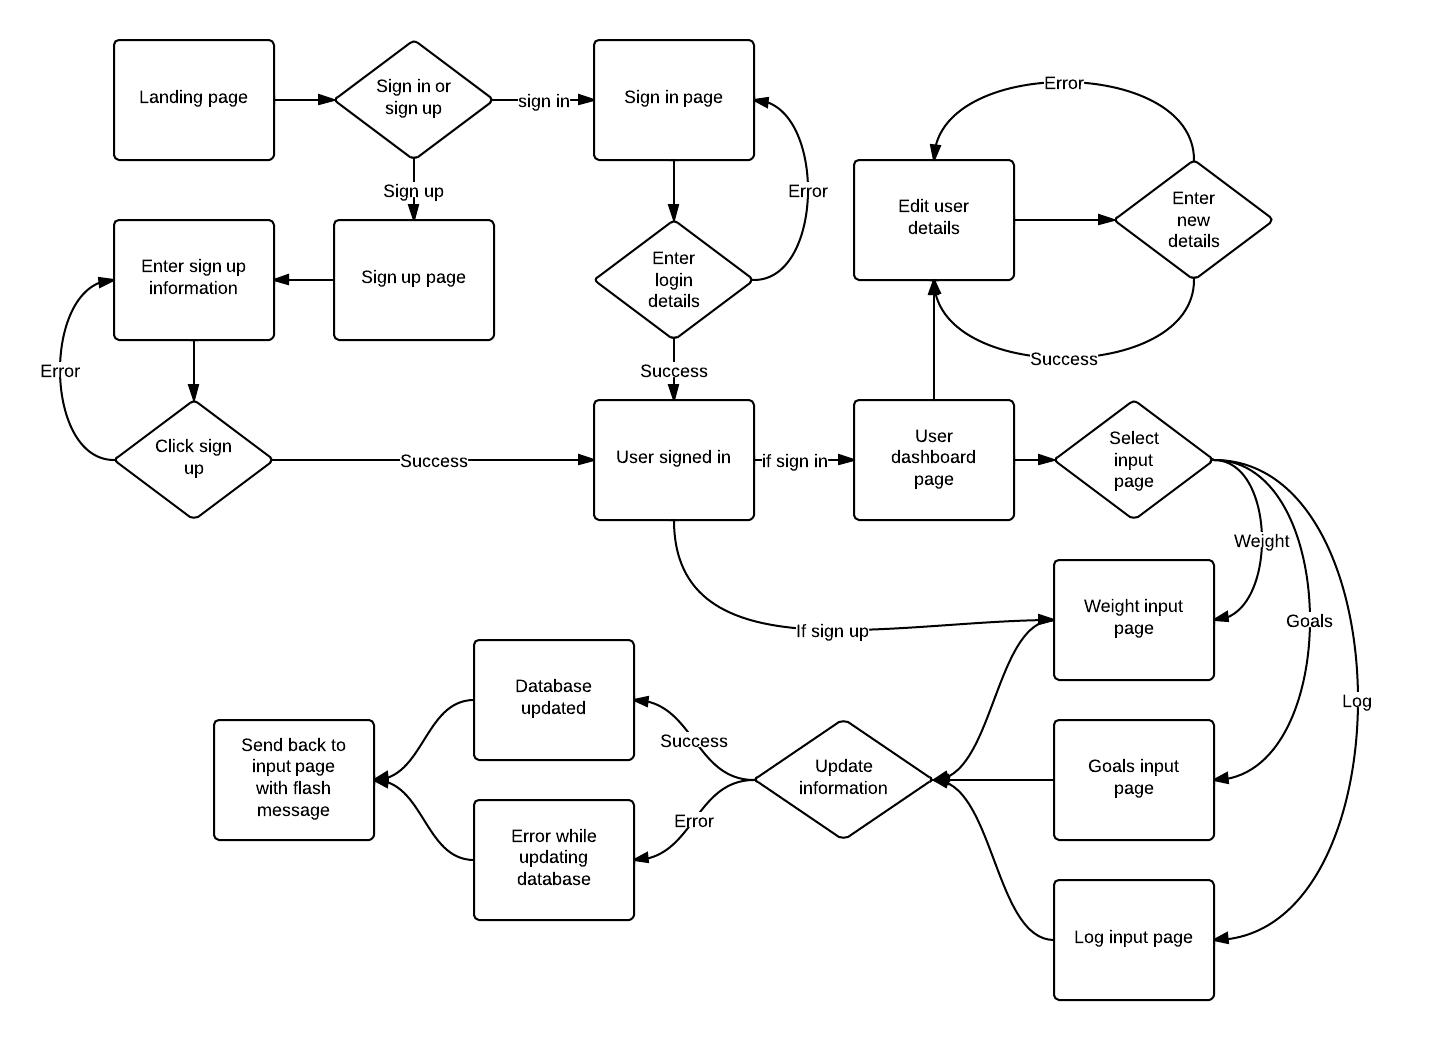
\includegraphics[scale=0.2]{chapters/figs/flowchart}
\caption{Flowchart for the processes and actions of the web application recur.}
\label{fig:flowchart}
\end{figure}

\subsection{Design in the browser}
Most of the design for the application was drawn up, but some of the easier designs were made directly in the browser. This was to speed up the process by cutting out unnecessary tasks. As opposed to the original plan, development begin during the design stage. This was because there was enough of a design to begin developing some of the application. Once development was underway some things had not been designed yet, for examples; the forms for signing in and out. There was a clear vision of what the forms should look like, so instead of wasting time making the wireframe and mock up of them, they were just designed on the fly, in the browser. This allows for rapid prototyping of the applications looks and lessens the work load on the design front, and even if the design does not work there is no reason why another design cannot be drawn up and implemented.\\

\subsection{Database design}
As well as design the application, the design of the backend will need to be done before development takes place. For the backend, Ruby on Rails \citep{rails:2013} will be used. Reasons for this will be discussed in the development chapter \ref{dev} page \pageref{dev}. A number of attributes will be store about the user and will be split up over a number of tables all with a one to many relationship to the user table. The other tables will be current weight, which will store the current weight of the user, goal weight, which will store the goal weight of the user, fitness log, which will store information about what exercises they did and how they did, and the goals table, which will store the users goals. All of these will link back to the users ID. Originally, there was going to be a user?s weight table, which store both the current and goal weight but it was moved to two different tables because it is unlikely that the user will be updating the goal weight as much as they were going to update their current weight. All of these tables will have depend upon their user, so if the user is removed from the database so will all their data. Below (Figure \ref{fig:erd}) you can see the entity relationship diagram for the application.

\begin{figure}[!ht]
\centering
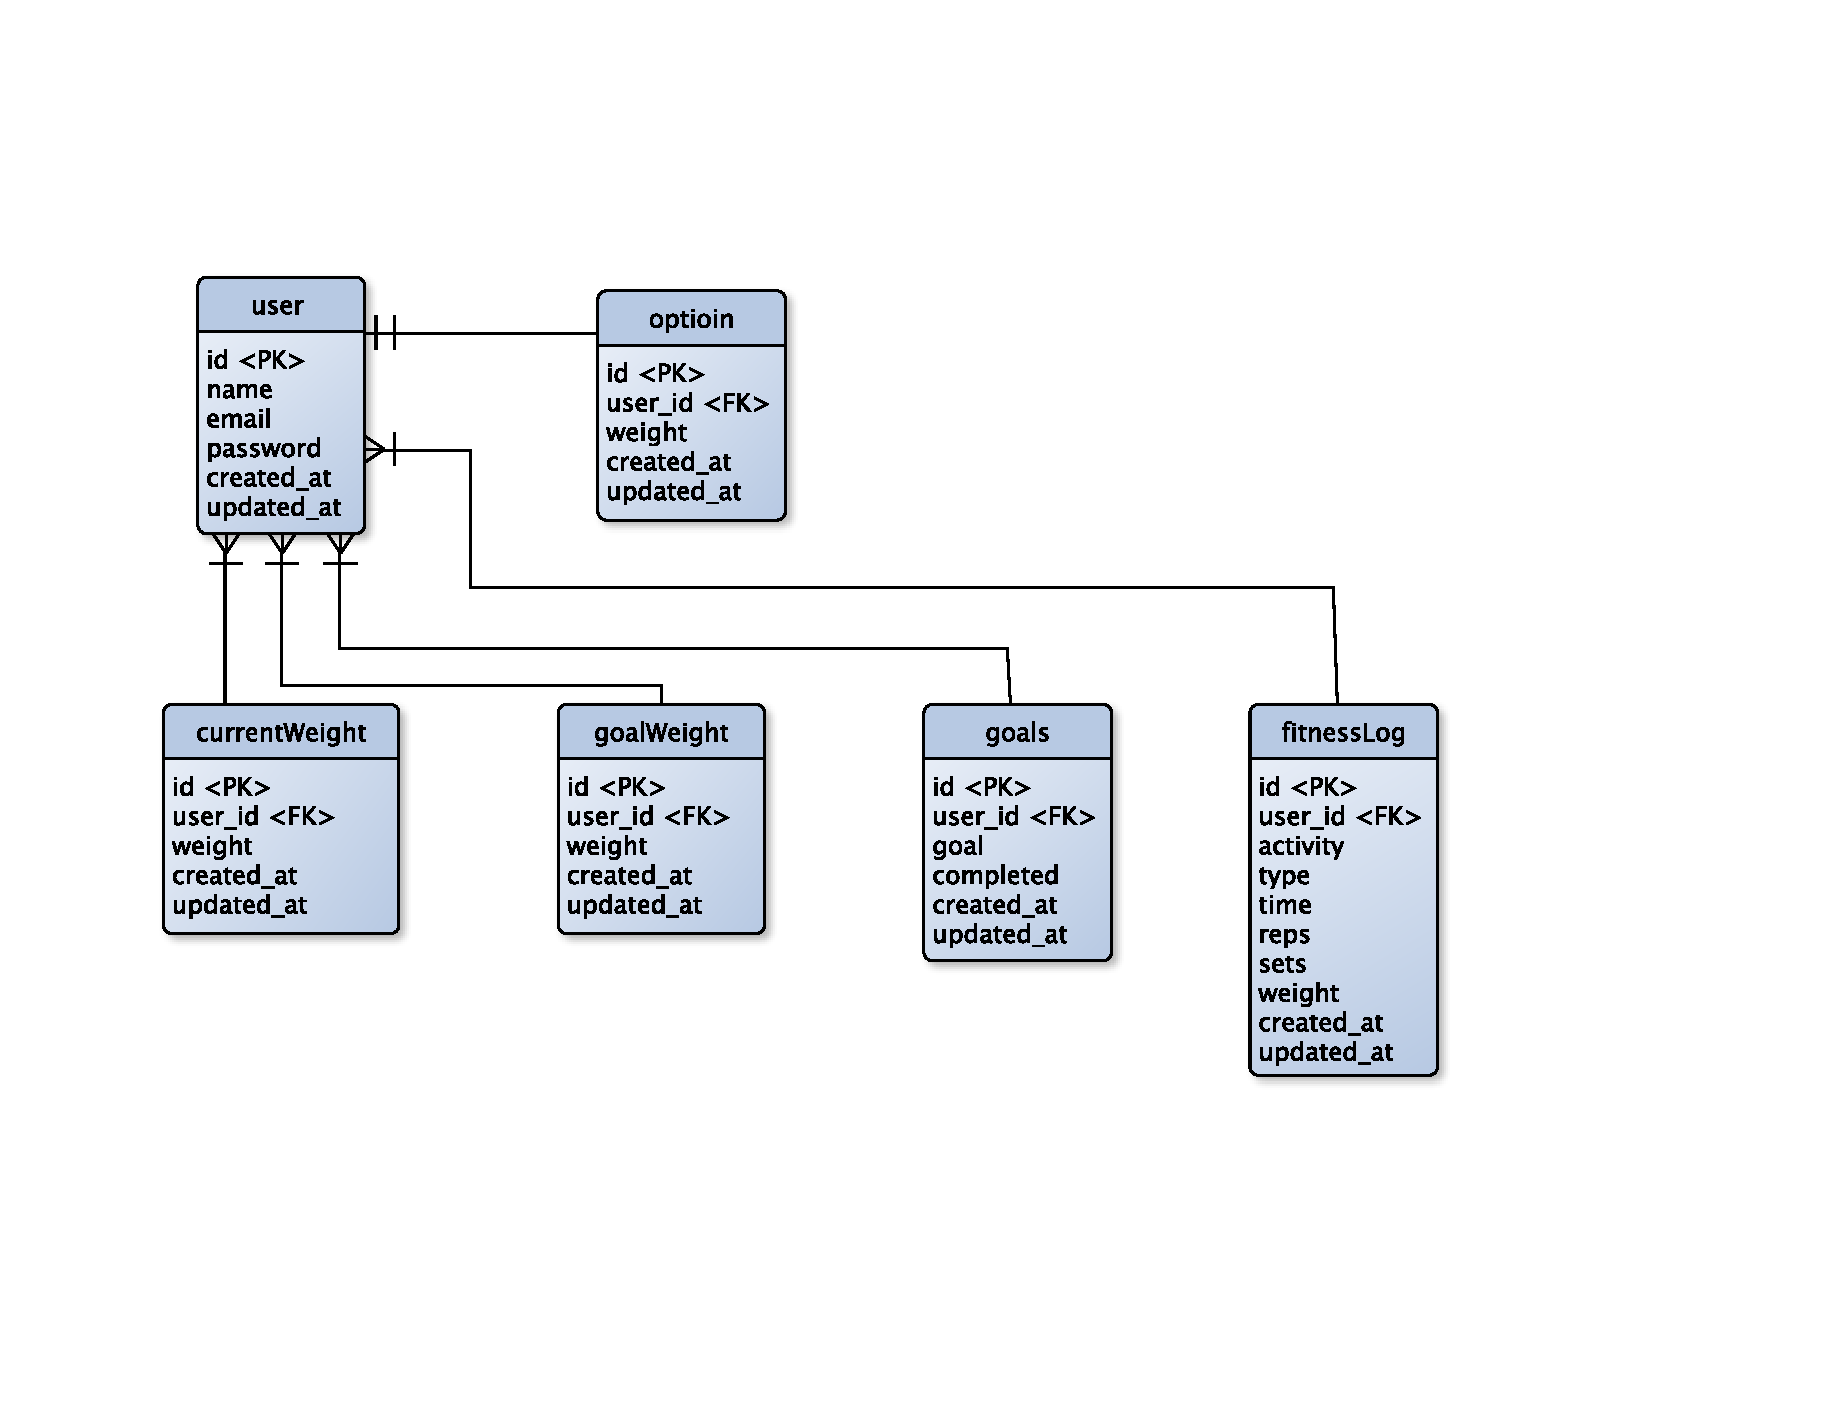
\includegraphics[scale=0.5]{chapters/figs/erd}
\caption{Entity Relationship Diagram for the website application recur.}
\label{fig:erd}
\end{figure}

\chapter{Resources}
\label{sec:resources}
\section{Introduction}
This chapter will talk about all of the resources that were used during the development of Recur. It will go into detail about the languages used, which applications were used, and also what RubyGems were used. It will talk about why each was used against its competitors.

\section{Languages and Frameworks}
\subsection{Ruby on Rails}
Ruby on Rails was the main backbone to this application. It was chosen for its rapid development characteristics, its extendability with the mass amount of Gems that can be easily added into a project, and its scalability when it comes under heavy load with lots of traffic. It was also chosen on personal preference as compared with other languages that have similar frameworks. There is not much difference between a framework written in Ruby and one that is written in PHP. They are both going to do the same job but someone will find it easier to write in Ruby and other will find it easier to write in PHP. The main point is the use of a framework at all. MVC frameworks provide a really good backbone to any application. The MVC framework is comprised of three components; the model, the view, and the controller. Each component has a specific task to take care of. In Ruby on Rails's case, the model is what talks to the database. It can enforce rules on the data coming into the database. For example; it must contain an email that is valid against a certain regular expression. The controller is the logic behind the application. It contains functions that link to the views of the application which will display the information. They also allow for rapid development of applications by using a system called CRUD \nomenclature{CRUD}{Create, Read, Update, Destroy}. CRUD stands for create, read, update, and destroy. Each controller in Rails will use these four methods to create, read, update, and destroy a record of the model in the database. Instead of having to make your own CRUD system, Ruby on Rails gives you a number of calls that does it all for you. This is much easier and quicker than writing it all yourself.\\

\subsection{JavaScript and jQuery}
jQuery is a JavaScript library that allows developers to do very complex JavaScript functions with very little code. jQuery makes it really easy to interact and manipulate the web page. This means we can show and hide elements based on what they user has input in a box, or checked off in a check box. The main use for jQuery was the hiding of elements in forms and showing the menu on small screen devices. It was also used for the chart switching on the fitness log. This will be explored in more detail later in this chapter. jQuery is also used for its AJAX method. AJAX is really useful when you need to update a database without refreshing the page. This was used when checking off goals. When it comes to alternatives to JavaScript and jQuery there are none. JavaScript is quite unique in that it is the only language that allows developers to manipulate the webpage while it is in use. With the progression to CSS3, developers can now do some page manipulation with that using element selectors and change style attributes on click and hover, but not to the extent that jQuery can.\\

\section{Tools}
A number of tools were used during development, some were used more than others but all of them played a key role in development. The main tool that was used is Sublime Text 2 \citep{sublimetext:2011}. This was the text editor that was used to build both the static mock up of the site and the full functioning web application. Sublime Text was chosen because of its vast amount of plugins. This makes it very versatile and efficient when it comes to building productions applications. There were a number of other editors considered for the job, for example; Vim \citep{vim:2013} was going to be chosen due to its rapid development capabilities from all of the navigation being done on the keyboard. But it was not chased due to the steep learning curve as this would eat into development time. The time investment into learning Vim would probably not be beneficial to such a small project but could be considered for future projects.\\

During the development of the static site, a JavaScript task runner called Grunt. It was used to compile Sass \citep{sass:2006}, minify javaScript, and optimise images. When development moved onto Rails it was dropped as Rails compiles Sass and minifies JavaScript in the assets pipeline.\\

The second main tool that was used was iTerm 2 \citep{iterm:2011} using the oh-my-zsh \citep{zsh:2009}. Using the command when building a Ruby on Rails application is absolutely necessary. It is used to generate controllers and models, start the Rails server, interact with the database, and a number of other key features. The terminal emulator is not really that important but the use of the Zsh shell was very useful to the development stage. It has a number of excellent features like displaying the current Git \citep{git:2014} branch that I was working in and if there was any changes that have not been committed and also highlighting in the terminal. Seeing as a lot of the time was spent in the terminal, it was important to make that time as productive and as efficient as possible.\\

Git was another tool that really helped with development. Git is a version control system. It allows the developer to commit files, and revert back any changes if something goes wrong. A slightly adapted branching methodology was used called Gitflow \citep{gitflow:2010} which allowed easier version control during development and having a live and stable master branch that could be used to push to Heroku.\\

Heroku \citep{heroku:2007} was used to host the site, more information on this service can be found in the deployment section \ref{sec:deployment} of this chapter on page \pageref{sec:deployment}.\\

An application called Dash \citep{dash:2014} was also used during development. Dash allows you to download documentation for certain languages and frameworks and stores it offline. It allowed the Rails documentation to always be readily available whenever.

\section{Gems}
RubyGems \citep{rubygems:2009} is a package manager for the distribution of Gems. A Gem is a small package of Ruby code designed to either work on its own, for example a to-do list keeper, or work inside another application, for example the LazyHighCharts gem that was used to add charts to the log section of the website. They can be very useful by cutting down the amount of code needed to be written or by already having complex function built in and therefore not having to write them yourself. A number of other Gems were used during development, along side the default Rails Gems. The bcrypt-ruby gem was used for user creation and authentication. It allows you to create a password digest for storing in the user's record using one way encryption. This makes the system a lot more secure than storing the password in plain text, or even using a salt and hash to store the password. Sass-rails was used so that the style sheets could be written in Sass and compile to CSS at build time. Sass is has a number of benefits over vanilla CSS, like being able to use variables for colours to allow for easier mass colour change. Better errors gem was also used during development to give a more in-depth error message when something went wrong. The default Rails error message is as descriptive as the better errors Gem so it becomes a lot easier to debug the application.\\
A number of testing gems were used during development to ensure the application was secure and working correctly. Rspec is the main gem which is used to write and run all of the tests. Using Rspec in conjunction with Capybara and FactoryGirl, it is easy to write extremely powerful tests. These tests not only interact with the Rails backend, but interact with pages and makes sure the redirects are working as intended.

\section{Conclusion}
To conclude this chapter, it is necessary to state that the outcome of the product will not be defined by the tools you use. Most tools are very similar and it almost always down to personal preference. However, in some circumstances, some tools will be better for a specific task than others.

\chapter{Development}
\label{sec:dev}
\section{Introduction}
This chapter will discuss the development stage of the production of the progress monitoring web application. It will cover a number of topics, from development tools used during this stage to development methods uses whilst building this application. It will also walk through, step by step, of the building process highlighting problems and how they were overcome.\\

\section{Tools}
A number of tools were used during development, some were used more and others but all of them played a key role in development. The main tool that was used is Sublime Text 2 \citep{sublimetext:2011}. This was the text editor that was used to build both the static mock up of the site and the full functioning web application. Sublime Text was chosen because of it is vast amount of plugins. This makes it very versatile and efficient when it comes to building productions applications. There were a number of other editors considered for the job, for example; Vim \citep{vim:2013} was going to be chosen on due to its rapid development capabilities from all of the navigation being done on the keyboard. But it was not chased due to the steep learning curve as this would eat into development time. The time investment into learning Vim would probably not be beneficial to such a small project but will be a consideration for future projects. During the development of the static site, a JavaScript task runner called Grunt. It was used to compile Sass \citep{sass:2006}, minify javaScript, and optimise images. When development moved onto Rails it was dropped as Rails compiles Sass and minifies JavaScript in the assists pipeline. The second main tool that was used was iTerm 2 \citep{iterm:2011} using the oh-my-zsh \citep{zsh:2009}. Using the command when building a Ruby on Rails application is absolutely necessary. It is used to generate controllers and models, start the Rails server, interact with the database, and a number of other key features. The terminal emulator is not really that important but the use of the Zsh shell was very useful to the development stage. It has a number of excellent features like displaying the current Git \citep{git:2014} branch that I was working in and if there was any changes that have not been committed and also highlighting in the terminal. Seeing as a lot of the time was spent in the terminal, it was important to make that time as productive and as efficient as possible. Git was another tool that really helped with development. Git is a version control application which allows the user to commit versions of code so that it would be easy to revert back to a previous version of code if something went wrong with development. A slightly adapted branching methodology was used called Gitflow \citep{gitflow:2010} which allowed easier version control during development and having a live and stable master branch that could be used to push to Heroku. Heroku \citep{heroku:2007} was used to host the site, more information on this service can be found in the deployment section \ref{sec:deployment} of this chapter on page \pageref{sec:deployment}. An application called Dash \citep{dash:2014} was also used during development. Dash allows you to download documentation for certain languages and frameworks and stores it offline. It allowed the Rails documentation to always be readily available whenever.

\section{Gems}
RubyGems \citep{rubygems:2009} is a package manager for the distribution of Gems. A Gem is a small package of Ruby code designed to either work on its own, for example a todo list keeper, or work inside another application, for example the LazyHighCharts gem that was used to add charts to the log section of the website. They can be very useful by cutting down the amount of code needing to be written or by already having complex function built in and therefore not having to write them yourself. A number of other Gems were used during development, along side the default Rails Gems. The bcrypt-ruby gem was used for user creation and authentication. It allows you to create a password digest for storing in the user\'s record using one way encryption. This makes the system a lot more secure than storing the password in plain text, or even using a salt and hash to store the password. Sass-rails was used so that the style sheets could be writing in Sass and compile to CSS at build time. Sass is has a number of benefits over vanilla CSS, like being able to use variables for colours to allow for easier mass colour change. Better errors gem was also used during development to give a more in-depth error message when something went wrong. The default Rails error message is as descriptive as the better errors Gem so it becomes a lot easier to debug the application.

\section{Development Log}
Development began ahead of schedule because designs were already done. Even though not all the designs had been done, the essentials were there, it was only separate pages that were missing. The colour scheme, font choice, and general feel were all there so development got started with the static HTML being built. Using Grunt \citep{grunt:2013} and sublime made getting out a static site very quick and easy. This stage did not take as long as I had originally planned. It was done within three days, where as originally it was to take two weeks. However, design has not being fully completed, what is commonly known as designing in the browser took place. This is where a rough idea of what the page is to look like is in the developer head and they just design it in HTML and CSS straight away, without going through the step by step process of wire framing and mock ups. While this is not a good idea on large scale project, the minimalist design that the application was adopted made it almost easier to design in the browser than draw wireframes and create mock ups.\\

Once the static site had been generated and the designs had been finalised it was straight into Rails development. The develop was split up into features and each feature was implemented separate. This allowed deadlines to be made so it was easy to track the progress and see if development was on track. The features that were split up were;

\begin{enumerate}
\item A user system with the ability to create a new user and login and out
\item Weight tracking, for both current and goal weights
\item Fitness log
\item Goal tracking
\end{enumerate}

\noindent
Once these deadlines were confirmed, development could properly begin.\\

Not much knowledge was known about Ruby on Rails was known before development, other than some basic syntax and that it is an MVC framework. So at first, the approach was to learn and build at the same time. This lead to two things and the first problem; it was very slow and the code was getting sloppy. This type of development style did not last very long when development came to a stand still when trying to implement the weight tracking. The decision was made to halt development and take the time to learn some Rails.\\

Two main sources for learning rails were used. The first one was a tutorial by Marc Someone. This tutorial took you through making a Twitter \citep{twitter:2006} clone. It was useful because it went through how to create a authentication/authorisation system, create relationships between the user and other models, and also some test driven development. The second was the Rails tutorials. These covered pretty much all parts of Rails so they were referred to as and when there was a problem that could not be solved by referring to the documentation. The Rails Documentation was also referred to a lot during development.\\

After a firm understanding of Rails was gained, development could continue. The downside to this break meant that development was now far behind schedule. As development went on though, it caught itself up. The learning break was worth it because development began to speed up and the code that was being produced was to a higher standard.\\

So far, only the user system had been implemented and it was time to move on to the weight tracking. This was were the problem of not knowing enough Rails to continue arose, which was solved with taking the time to learn it instead of learning as development went on. So when it was time to come back to it, all the weight tracking code that was used prior to learning Rails was removed. This was made easy with Git. Git allows you to reset changed to a certain commit. The code was rolled back to where the user system was just finished and so was the Rails database. For the weight tracking, two separate models were used. Originally, the goal weight was going to inside the user model but the decision was to split it off was so that it could possibly used for future analysis. For example; plotting a graph for both the users weight and their goal weights against time so they will be able to see when they hit their goals. This also lead to splitting up the goal weight and the current weight into tables. Another factor into this was the thought that user will be updating their current weight much more than their goal weight. So to have them in the same table would lead to multiple duplicate goal weights. These weight were to be shown on the dashboard and updated through a different page. In the original design, there was going to be a little graph under where the weights are displayed on the dashboard. This idea was removed because of how small the graph would be. It was moved to the weight input page so that it could be a lot bigger and the user would be able to gain more information from it. The weight input screen was kept really simple. It has two input boxes and two submit buttons, one for the goal weight and one for the current. Rails allows for very simple AJAX integration with forms. AJAX allows the user to update the database without having to leave the current page. This will allow the user to update their weights and then consult the graph without having to load the page again. It will be a great help on mobiles where the connection may not be great.\\

Once the weight tracking was implemented it was on to the next feature which is the fitness log. The fitness log is its own table which consists of six fields:

\begin{enumerate}
\item Activity - The name of the exercise
\item Type - What type of exercise (strength, cardio)
\item Time - How long the user spent doing the exercise
\item Reps - How many repetitions the user did
\item Sets - How many sets the user did
\item Weight - How heavy the weight was
\end{enumerate}

There are two main types of exercises; strength and cardio. There were two options when it came to storing this information. Option one was to have three tables; fitness log, cardio, and strength. The fitness log would just store the user\'s ID and the ID of either a cardio entry or a strength entry. Or option two which is to have them all one table and use some logic in the controller and view to determine what to do with the data dependant upon whether it is a strength exercise or a cardio exercise. The reason for needing to either split them up or use some logic is because a cardio exercise does not have any sets, reps or weight. They are usually a time based exercise. Whereas, its the other way around for strength training. The user will want to track their sets, reps, and weight, and not how long it took them to perform the exercise. The decision was made to keep them all in the same table because it was easier to implement. Both ways would need some logic at either the inputing into the database end or the extracting end. The logic that was used in the view controller for showing the fitness log was very simple. Thereiss a foreach loop that prints out the information and if the type was equal to cardio then it would print out the format ``Activity - time'', for example ``Cycling - 120 mins'', and if it was strength it would print out ``Activity - sets*reps @ weight'', for example ``Bench press - 3*6 @ 160 lbs''. There is also some logic in the controller that groups the entries by date, so that all the entries for that day will be grouped together.\\

The application would have suggestions for exercises activities. This was for the same reason has having the drop down menu on type, to add consistency to the inputs and throughout the records in the database. Originally, the suggestions were hardcoded into the HTML using the datalist attribute in HTML5 but then a better solution occurred. Having the list hardcoded in to the HTML meant that it was hard to update and keep on top off. Also, what happens if the user did something that was not on the list? If they did that again, what if they inputed it without capitals this time? While changing from capitalised to no capitalised will not break the application, it is better to have everything in the same format. The solution to this problem was to build the datalist from previous exercises the user has completed. This way, if the user has does a certain exercise repeatedly that was not on out list, they will still get the autocomplete function.\\

As well showing a list of all the of the exercises that the user had completed that day, the application will need to show the users progressing through their time using recur as this was one of the main goals to keep the user motivated by showing them their progression. Three charts were added to the log view of the website to show their progression on the three main compound weight lifting exercises; the bench press, the deadlift, and the squat. The charts were added using highchart.js \citep{highcharts:2009}. A helper gem called LazyHighCharts \citep{lhc:2010} was used so that the chart could be built in the controller of the application instead of being built in JavaScript in the view of the application. Using the gem made the code a lot easier to manage and change.

Once the fitness long was done, the date card could be worked on. At first, the date card was just going to display the current date but the box looked very empty and out of place. To add motivation to the card, a ``time since last gym visit'' was added to this card. This would work in two way.

\begin{enumerate}
\item Motivate them to keep this time down to as little as possible by getting into the gym as often as they could.
\item Motivate them to get back into the gym after a long break by reminding them that they have not been in a long time.
\end{enumerate}

Using Rails today \lstinline{Date.current()} function to get the current date and the \lstinline{Created_at()} date from the last fitness log entry from the current user, the application was able to figure out how long it had been since the users last gym visit. Rails also has another great function for this which is \lstinline{distance_of_time_in_words()} which takes in two date functions and prints out the distance is real words. For example: less than a minute since your last visit to the gym. or 5 days since your last visit to the gym..\\

After the date card, there was only one feature left to implement. This was the goals feature. Goals was a table that stored two values; the goal and complete. Goal was a string and was what the goal was, and complete was boolean. Goals are shown on the dashboard and can be inputed from the \lstinline{goals_user_path(current_user)} in the Rails application. Goals was not a very hard feature to implement. It was simply just one form that created the element and then a list the showed all the goals with a checkbox to check the goals off. Where it got difficult was with AJAX. I wanted the goals to be updated using AJAX, both inputing the goal and checking the goal off. When using AJAX to input the data, I was running into all sort of trouble. At first, it would input the goal multiple times, and then it would not update the last properly when the goal at been input. The decision was to move this to a could have priority. As for checking the goals off, the AJAX works really well. The user will check the box, the goal will then turn red and have strikethrough. After a second the goal will fade and update the record by setting complete to true. Currently, there is no way to uncheck the goal and get it back, the user will have to input. The completed goals are shown below the current goals and they also display their completed on date. With the way the grid works to make the website responsive, on the goals page it will put the first goals card above the input card. This will cause a big problem if the user has a lot of completed goals. To fix this problem, the list will be hidden when the display size is under 650 pixel and a jQuery function will be added to the display this and hide it again.\\

Now that all the main features are added and a working prototype is complete, all that needs doing now is tidying up. The development stage was still a learning process, so a lot of corners were cut. Mainly on aspects like styling and the feel of the website. So now development will continue by tidying up the lose ends of the application with things like, fixing the responsiveness of the website so that it completely mobile friendly, and making sure the flashes show when the user submits by AJAX.\\

After everything was done, it was apparent that there was no way to analysis the data as an admin. This was resolved by added an access attribute to the user, that would default to zero. If the access of a user was changed to one, then they would have access to the admin panel. The admin is able to see a list of all the users, along with their current and goals weights, how many goals they have against how many they have completed, how many times they have updated their fitness log, and when they last updated their fitness log. They will also be able to view users pages but not update their information. \\

\section{Clean up}
Once all of all the main features were implemented, a clean up took place. This meant doing things like catching bugs and fixing them that the testing did not pick up, making sure the correct flash displayed with the correct styling, and making sure that the website was accessible from all devices. Most of these had already been picked up during development so there was not a lot to do when it came to cleaning up. The main problem was the flashes. If the form was submitted through AJAX, then the flash would not show, but it would show on the next reload. This was fixed by moving the flash over to a partial and rendering the partial at the top of the page, and then when the AJAX javascript was called, it would update the flash and any other part of the webpage that needed to be dynamically updated. This also solved another problem of having a lot of repeated code. The way to display a flash is the same on every page, and it was repeated on almost every page. Moving it over to partial cut down the code per page.\\

\section{Optimisation}
Optimisation is a big part of todays web industry. With a lot of people browsing the web from their mobiles, their download speeds are slower than broadband speeds. They also have data caps which restrict the amount of data one user can download in a month. There are certain steps that can be taking to reduce the time it takes for a user to load up the webpage on their mobile devices. The first way we can do this is by manipulating the JavaScript and CSS files. HTTP request will slow down the page the load time so we can concatenate the JavaScript and CSS files to reduce the number of HTTP requests we are calling per page. We can remove all of the unnecessary whitespace from this files. This process is called minification. Using both concatenation and minifcation of files, you stand to reduce a large chunk of requests from your website, improving your load time. Other options include optimising your images. Images are the biggest item to load on webpages, ranging from kilobytes to a few megabytes each. There are lots of tools to use for optimising your images. ImageOptim \citep{imageoptim:2014} is what was used for optimising the images. Because not many images are used it wasn't necessary to go through all of the image optimisation steps. ImageOptim gave enough results to justify not going further with image optimisation.\\


\section{Deployment}
\label{sec:deployment}
Deployment of the web application was done through a service called Heroku. It offers a free hosting services for small application but will automatically scale up when demand for the website rises. This was perfect for the application as it was easy to get a prototype on the web quickly but if demand for the website rose then Heroku would scale up my application to match the demand. It was also chosen for its ease of use. It ties in well with Git and just creates a new remote in your local repository to push to. It will thens detect what type of application is being deployed, a Rails application in this case, and do all the setting up necessary to a Rails application. The only setup needed on our end was a few changes to the gem file. Adding a production and development group to switch between a MySQL \citep{mysql:1995} for local testing and PostgrepSQL \citep{postgres:1995} database for Heroku, and adding the Git remote which was made simple with the Heroku tool belt. Heroku also has the option to allow to assign your own domain to it.\\

Other options were to deploy to a virtual Private server using the Capistrano gem \citep{capistrano:2013}. This was the original idea but after discovering Heroku it seemed slightly overkill. Also, with Ruby applications, dependences have to match up, other wise your application will not run. While you can force gem versions in the gem file, Heroku manages all that for you.


\chapter{Testing and Evaluation}
\label{sec:test}
\section{Introduction}
This chapter will cover the testing of application. It will go into detail about the choices made and give reasons as to why certain tools or methodologies were used over others.\\

\section{Methodologies}
For the main part of testing, test driven development(TDD) was used throughout the building of the application. TDD was used because of the constant deployments to Heroku. All of the features implemented had to be working perfectly before deployment. Sometimes this was not the case though. All of the tests are written so sometimes you miss a test case and this can lead to deploying broken code. Usually, most of the bugs were picked up either by the testing or quite quickly after deployment if any bugs got through. TDD fitted in well with the Agile development approach that was taken when building the application. TDD and Agile development were used to make testing easy. TDD tests the code as you are working so you are not left doing all the test last, or after every feature. This allowed to get working prototypes out and deployed very quickly.\\

\section{Tools}
\subsection{Rspec}
\subsection{Chrome Development Tools}

\section{First release}
March 11th 2014 marked the first release of recur. It was posted to the fitness subreddit of the popular image board site Reddit\citep{reddit:2005}. The idea was to do a small release to pick up on any bugs that got through testing. It became very helpful because as the developer of the site knew how everything worked because they had built it, other people said they did not know where to click. This subject had been raised by colleague and fixed with an image of a chain link to denote a link. After this feedback had been submitted, changes were made to the title links. They were made more obvious when rolled over with a background colour change and also, if it is the users first visit to the site then they will be shown a message telling them that the titles of the cards are links to more information. Other feedback included users receiving error flashes when really the database was successfully updated. This was because the error flash was getting called if the log entry was saved or not. This caused uses to submit multiple entries to the database for the same activity. This then caused another problem of not being able to removed a logged activity after it was put into the database. An obvious feature was overlooked during development but was soon implemented in to make sure users could delete unwanted logged activities. The way the log was displayed was also rewritten to make it easier to see which data went with which activity. Users also wanted to be able to see which goals they had completed on the dashboard. This was limited down to goals that had been completed in the last 2 weeks.


\section{Conclusion}

\chapter{Conclusion}
\label{sec:conc}
\section{Learnings}
The outcome of building this design has been a great help for me personally. It gave me the opportunity to learn a lot about what goes into an application that has the potential to gain lots of users. The design process taught me lots about designing for user accessibility. Before, when designing my application, it was all about appearance. But now I understand that there is more to web design than just aesthetics. It is important that the user is able to use the application easily without much hand holding. The design should ease users towards where they need to go, not just expect them to know exactly how to use it straight away. Also, some users may be visually impaired. This has the potential to cause a lot of problems when they're using the website. If you have not catered for them, it could be impossible for them to interact with the website. This is a major problem as you are alienating a large percentage of the population. On a similar note, being able to support a multitude of browsers and devices is important. As mentioned in the report, with mobile traffic increasing it is very important that the application has the same functionality on mobile as it does in the browser. And across all browsers, not just the main ones. The last thing I learnt was that mock ups are important. I never used to think that they were and I would just jump straight into the browser, but with this project I found that they are a great help to have something to refer to instead of having to think up where you are going to put element X.\\

Development taught me that having an understanding of the tools you are going to be using is very important. I went in with very little knowledge of Ruby on Rails and my project was set back many weeks because of it. I will, from now on, make sure that I have a good understanding of everything that will be involved with my project before I undergo any serious development. The pause in the middle of development to go away and learn the language was a massive set back. If I could go back and do this again I would spend the first few weeks gaining knowledge of the tools and technologies I would be using. Also, I had to learn about security and keeping my users safe from attackers. I was lucky enough to have a lot of the functionality from other tools (bcrypt, PostgreSQL hosted on Heroku) that I did not need to worry about it so much, but it was still something I had to take into consideration.\\

During testing I found that it is very important to test from the very beginning. I was not using test driven development at the beginning and it was taking a very long time to make progression because I was finding bugs all the time in previously written code. Once I implemented test driven development, progression sped up and I was able to rapidly progress through and get a releasable product. I also learnt that you can only test so much. Even thought I had been testing thoughout development, upon first release almost every user had found a bug. Whilst this was not ideal, it was certainly helpful that they reported it. At first, I was using the built in Rails testing framework which I found to be restricted and not as simple as what I had seen form Rspec. As soon as I switched over to Rspec I found that I was writing test much quicker and it was easier to debug when an error was found. If I was to start again, I would definitely use Rspec from the beginning.

\section{Future plans}
I plan to maintain Recur for the foreseeable future. I feel it has potential to become something useful for a broad portion and a variety of society. The application could use a new design. Whilst I am satisfied with the design and I think that it for fills its purpose, it definitely needs reworking in some parts. Also, some of the code could use refactoring. While this is not a major issue, if I was to ever sell this on to someone else, having a clean, commented, and well documented code base is very important. \\

Another project that could happen with this application is the development of an iOS or Android application. One of the great things about Ruby on Rails is that it is very easy to extend the functionality of the web application to an API. This will then allow me to develop a mobile application that will make calls to Recur\'s API so the users will be able to retrieve and update their information from a native mobile application. Seeing as one of the main goals is to make sure that the application works in mobile browsers and the main use of this application is to update your fitness log on the go, it would make sense for a native mobile application to exist. 

\pagebreak
\renewcommand{\bibname}{References}
\addcontentsline{toc}{chapter}{References}
\bibliography{bib}

\end{document}